\documentclass[11pt]{article}

% ---- geometry / typography ----
\usepackage[a4paper,margin=1in]{geometry}
\usepackage{lmodern}
\usepackage[T1]{fontenc}
\usepackage{microtype}
\usepackage{parskip}
\setlength{\parindent}{0pt}
\setlength{\parskip}{0.5\baselineskip}

% ---- math and graphics ----
\usepackage{amsmath}
\usepackage{amssymb}
\usepackage{graphicx}
\usepackage{float}

% ---- captions and links ----
\usepackage[font=small,labelfont=bf,labelsep=period,margin=1cm]{caption}
\PassOptionsToPackage{hyphens}{url}
\usepackage[hidelinks]{hyperref}
\usepackage{xurl}
\hypersetup{colorlinks=true,linkcolor=black,citecolor=black,urlcolor=blue!60!black,breaklinks=true}

% ---- section spacing ----
\usepackage{titlesec}
\titleformat{\section}{\Large\bfseries}{\thesection}{0.8em}{}
\titleformat{\subsection}{\large\bfseries}{\thesubsection}{0.8em}{}
\titlespacing*{\section}{0pt}{1.6\baselineskip}{0.6\baselineskip}
\titlespacing*{\subsection}{0pt}{1.1\baselineskip}{0.4\baselineskip}

% ---- consistent figure width ----
\newcommand{\figw}{0.85\linewidth}
\newcommand{\figwide}{0.95\linewidth}

\title{\vspace{-1cm}\textbf{From Brownian Paths to the Heat Equation}\\[0.3em]
       \large Two Numerical Routes to Black--Scholes}
\author{Dorian Przetakiewicz}
\date{06.\ February 2026}

\begin{document}
\begin{titlepage}
\maketitle
\thispagestyle{empty}
\vspace{2em}
\begin{abstract}
\noindent
This project prices vanilla and exotic European options in two independent ways: a Monte Carlo simulation based on the Feynman--Kac representation, and a numerical solution of the Black--Scholes equation cast as a heat equation via an operator-splitting scheme. Both approaches are cross-checked against known analytical formulae. The Monte Carlo section covers European, Asian, binary and lookback options. The diffusion section presents the reduction to the heat equation, a Strang-split time evolution, and a comparison to the analytical call surface both for a short-maturity market option and for a longer-maturity benchmark.
\end{abstract}
\end{titlepage}

\pagenumbering{roman}
\tableofcontents
\clearpage
\pagenumbering{arabic}
\setcounter{page}{1}

\section{Monte Carlo Simulation of the Black--Scholes Formula}
In order to do a Monte Carlo simulation with the goal to calculate option prices, we make use of the so-called Feynman-Kac formula. The Black Scholes formula is given in \ref{eq:bs}. The Feynman Kac formula applies to PDE's (like the B-S) of type,
\begin{equation}
    \frac{\partial C}{\partial S}a(S,t) + \frac{1}{2}\frac{\partial^2 C}{\partial S^2} b(S,t)^2 + \frac{\partial C}{\partial t} - r(S,t)C = 0
    \label{eq:kacreq}
\end{equation}
with final condition $C(S,T) = C(S)$ and $dS = a(S(t),t)dt + b(S(t),T)d\tilde{W}$. Applying that to the Black-Scholes formula, we receive:
\begin{equation}
    C(0) \equiv C(S,0) = \langle e^{-rT} C(S(T)) | S(0) = S_0 \rangle_{\mathcal{\tilde{P}}}
\end{equation}
where $S_0$ is the current share price and $\mathcal{\tilde{P}}$ the martingale probability measure, under $C_{B-S} = \langle PV(C(T))\rangle_{\mathcal{\tilde{P}}}$.\\
From this one could derive the formula to calculate the current (european) option price like,
\begin{equation}
    C(0) = \int_{0}^{\infty} dS e^{-rT}C(S,T) \frac{1}{S\sqrt{2\pi \sigma^2 T}} e^{-\frac{\left[ln(\frac{S}{S_0})-(r-\frac{1}{2}\sigma^2 T)\right]^2}{2\sigma^2 T}}
\end{equation}
meaning that for european options the payoff function $V(S,T)$ depends only on the share price $S(T)$ and we can calculate this numerically. \\
In the case of european options, put and call, the payoffs do not depend on the share price trajectories, thus inside a Monte Carlo simulation, we do not have to do $x$ time-steps, but can immediately calculate the sample $S(t+T)$ instead of x steps á $S(t+\Delta t)$. \\
We assume the price of the stock to behave like Geometric Brownian motion with drift $r$ and volatility $\sigma$:
\begin{equation}
    S(t+\Delta t) = S(t) e^{(r-\frac{1}{2}\sigma^2)\Delta t + \sigma \sqrt{\Delta t} \xi}, \quad \xi \propto \mathcal{N}(0,1)
    \label{mc:stockprice}
\end{equation}
Using this assumption and formula, we can also price exotic options like asian or lookback options.\\
So to realize the Monte Carlo simulation, we start at $t=0$ with $S(0) = S_0$ then we split the time $T$ into \textit{steps} (an integer) of size $\Delta t$. That way we generate $N_{MC}$ trajectories $\{S(t)\}$ in the range $0\leq t\leq T$. For each trajectory we compute the payoff, according to the options payoff functions as defined later, and finally we estimate:
\begin{equation}
    \langle e^{-rT} C(S(T))|S(0) = S_0 \rangle_{\mathcal{\tilde{P}}} \approx \frac{1}{N_{MC}} \sum_{i=1}^{N_{MC}} e^{-rT} C(S(T))_{i}
\end{equation}
In each step we generate a random number $\xi$. This random number is generated using the Mersenne Twister algorithm (\texttt{std::mt19937\_64}) under a normal distribution with $\mu=0$, $\sigma=1$.

The way i implemented this in C++ is, i created a class called \texttt{BlackScholes} which holds the following members:
\begin{center}
\renewcommand{\arraystretch}{1.2}
\begin{tabular}{@{}ll@{}}
\texttt{N} & $= N_{MC}$, number of Monte Carlo trajectories \\
\texttt{stepSize} & number of $\Delta t$ time-steps per trajectory \\
\texttt{type} & option type (asian, binary, european, lookback) \\
\texttt{X}, \texttt{r}, \texttt{sig}, \texttt{T} & strike, risk-free rate, volatility $\sigma$, maturity \\
\texttt{S0} & initial stock price $S_0$ \\
\texttt{S} & array of stock prices along the current trajectory \\
\texttt{payoffs} & array of payoffs, one entry per trajectory \\
\texttt{discounted} & discounted payoffs, $e^{-rT}\cdot\texttt{payoffs}$ \\
\texttt{dt} & $= \Delta t$, single sub-step size \\
\texttt{lastPrice} & pointer to the last entry of \texttt{S} \\
\end{tabular}
\end{center}

The member \texttt{type} selects the payoff function $F$, which differs both by option type (asian, binary, european, lookback) and by put/call. \texttt{S} stores the stock prices of the current trajectory and is used inside path-dependent payoff functions (e.g.\ the Asian options). For the European and binary options it is sufficient to use \texttt{lastPrice}, a pointer to the last entry of \texttt{S}. Finally \texttt{payoffs} and \texttt{discounted} store the (undiscounted and discounted) payoffs of each trajectory, from which we recover today's option price $C(S,0)$.
Finally we take the mean of all discounted option prices to calculate an estimate of the true option price:
\begin{equation}
    C(0) \approx \frac{1}{N_{MC}} \sum_{i=1}^{N_{MC}} e^{-rT} C(S(T))_i
\end{equation}
with the standard error:
\begin{equation}
    \sigma = \sum_{i=1}^{N_{MC}} \sqrt{\frac{(e^{-rT} C(S(T))_i - C(0))^2 }{n(n-1)}}
\end{equation}
\subsection{Option Types}
In my Monte Carlo simulation i simulate the following option types and compare them with their analytical solution.\\
\textbf{European Call}: Right to buy at strike X.\\
Payoff function:
\begin{equation}
    F(S,T) = \max(S_T - X, 0)
\end{equation}
Analytical function:
\begin{equation}
    C_{\text{Euro}}(S,T)=S_{0}N(d_{1})-X e^{-rT}N(d_{2})
\end{equation}
with
\begin{equation}
    d_{1}=\frac{\ln(S_{0}/X)+\left(r+\tfrac{1}{2}\sigma^{2}\right)T}{\sigma\sqrt{T}},\quad
    d_{2}=d_{1}-\sigma\sqrt{T}
\end{equation}
and (N is the CDF of the standard gaussian):
\begin{equation}
    N(x)= \Phi(x) = \tfrac{1}{2}\left(1+\operatorname{erf}\!\left(\frac{x}{\sqrt{2}}\right)\right)
\end{equation}
\textbf{European Put}: Right to sell at strike X.\\
Payoff function:
\begin{equation}
    F(S,t) = \max(X - S_T, 0)
\end{equation}
Analytical function:
\begin{equation}
    P_{\text{Euro}}(S,T)=X e^{-rT}N(-d_{2})-S_{0}N(-d_{1})
\end{equation}
\textbf{Asian Call} (arithmetic average): Depends on average stock price over the path.\\
Payoff function:
\begin{equation}
    F(S,T) = \max(\bar{S} - X, 0), \quad where (\bar{S} = \frac{1}{n}\sum_{i=1}^n S_{t_i}).
\end{equation}
Analytical function (taken from~\cite{divaAsian}):
\begin{equation}
    C_{Asian}(S_0, T) = \exp\left[((\rho - r)T) \right](S_0 \Phi(\tilde{d1}) - X \exp\left[(-\rho T) \Phi(\tilde{d_2}))\right]
\end{equation}
where (m is equal to the number of steps per trajectory)
\begin{align}
    &\sigma_z = \sigma \sqrt{\frac{2m+1}{6(m+1)}} \quad \rho = \frac{r-\frac{\sigma^2}{2} + \sigma_Z^2}{2}
\end{align}
and
\begin{align}
    \tilde{d_1} = \frac{\log{\frac{S_0}{X}+ (\rho + \frac{1}{2}\sigma_z^2})T}{\sqrt{T}\sigma_Z}, \quad \tilde{d_2} = \frac{\log{\frac{S_0}{X}+ (\rho - \frac{1}{2}\sigma_z^2})T}{\sqrt{T}\sigma_Z}
\end{align}
\textbf{Asian Put} (arithmetic average):\\
Payoff function:
\begin{equation}
    F(S,T) = \max(X - \bar{S}, 0), \quad where (\bar{S} = \frac{1}{n}\sum_{i=1}^n S_{t_i}).
\end{equation}
Analytical function:
\begin{equation}
    P_{asian}(S_0,T) = \exp \left[ (\rho - r)T \right] (X \exp \left[ -\rho T \right] \Phi(-\tilde{d_2}) - S_0\Phi(-\tilde{d_1}))
\end{equation}
\textbf{Binary Call}: Fixed cash if in-the-money.\\
Payoff function:
\begin{equation}
    F(S,T) = \Theta(S_T - X)
\end{equation}
Analytical function:
\begin{equation}
    C_{\text{bin}}(S_0,T)=e^{-rT}\Phi(d_{1} - \sigma\sqrt{T})
\end{equation}
\textbf{Binary Put}:\\
Payoff function:
\begin{equation}
    F(S,T) = \Theta(X - S_T)
\end{equation}
Analytical function:
\begin{equation}
    P_{\text{bin}}(S_0,T)=e^{-rT}\Phi(-d_{2})
\end{equation}
\textbf{Lookback Call} (floating strike): Payoff is the difference between price at maturity and the minimum value of the asset price over the duration of the option lifetime; formulae taken from~\cite{quantstartLB}.

Payoff function:
\begin{equation}
    F(S,T) = \max(S_T - S_{min},0)
\end{equation}
Analytical function:
\begin{equation}
    C_{\text{LB}}(S_0,T)=S_{0}\Phi(a_{1}(S,m))-m e^{-rT}\Phi(a_{2}(S,m))
    -\frac{S_{0}\sigma^{2}}{2r}\left(\Phi(-a_{1}(S,m))-e^{-rT}\left(\frac{m}{S_{0}}\right)^{\frac{2r}{\sigma^{2}}}\Phi(-a_{3}(S,m))\right)
\end{equation}
with:
\begin{align}
    &M= \max_{0\leq \tau \leq T}S_{\tau}, \quad m= \min_{0\leq\tau\leq T}S_{\tau}
\end{align}
where:
\begin{equation}
        a_{1}(S,H)=\frac{\ln(S/H)+(r+\tfrac{1}{2}\sigma^{2})T}{\sigma\sqrt{T}},\quad\\
\end{equation}
\begin{align}
    &a_{2}(S,H)=a_{1}(S,H)-\sigma\sqrt{T},\quad
    &a_{3}(S,H)=a_{1}(S,H)-\frac{2r\sqrt{T}}{\sigma}
\end{align}
\textbf{Lookback Put} (floating put):\\
Payoff function:
\begin{equation}
    F(S,T) = \max(S_{max} - S_T,0)
\end{equation}
Analytical function:
\begin{equation}
    P_{\text{LB}}=-S_{0}\Phi(-a_{1}(S,M))+M e^{-rT}N(-a_{2}(S,M))
    +\frac{S_{0}\sigma^{2}}{2r}\left(\Phi(a_{1}(S,M))-e^{-rT}\left(\frac{M}{S_{0}}\right)^{\frac{2r}{\sigma^{2}}}N(a_{3}(S,M)\right)
\end{equation}
\subsection{Results}
In the following i will present the results of the Monte Carlo simulations, compared with their analytical values. \\
In all simulations, except the lookback option simulations and the european call option simulation we use $N_{MC}= 100000$ and $n_{steps}=250$ $\Delta t$ time steps per trajectory.\\
\begin{figure}[htbp]
    \centering
    
\includegraphics[width=\figw]{plots/BKX_european_call.png}
    \caption{BKX European Call option with maturity date 2013-03-16, quoted on 2013-01-02. Bid: 13.1, Ask: 17.4; $N_{MC}=10000$, $S_0=52.93$, $X=37.5$, $r=0.01$, $\sigma=0.1586$, $T=17/365$; data from~\cite{optiondata}.}
    \label{eu-call}
\end{figure}
In Fig. \ref{eu-call} we see that the trajectory shows strong spikes in the beginning, this is because the running mean has less values to be computed on and thus shows a higher variance. In the next plots i will remove the first $20\%$ of data points to showcase the motion of the option price depending on the number of trajectories with a more stable running mean. \\
We see that the simulation returns an option price that is within the price regime (ask-bid) of the actual option, and has a deviation of $0.94\sigma$ to the analytical price.
\begin{figure}[htbp]
    \centering
    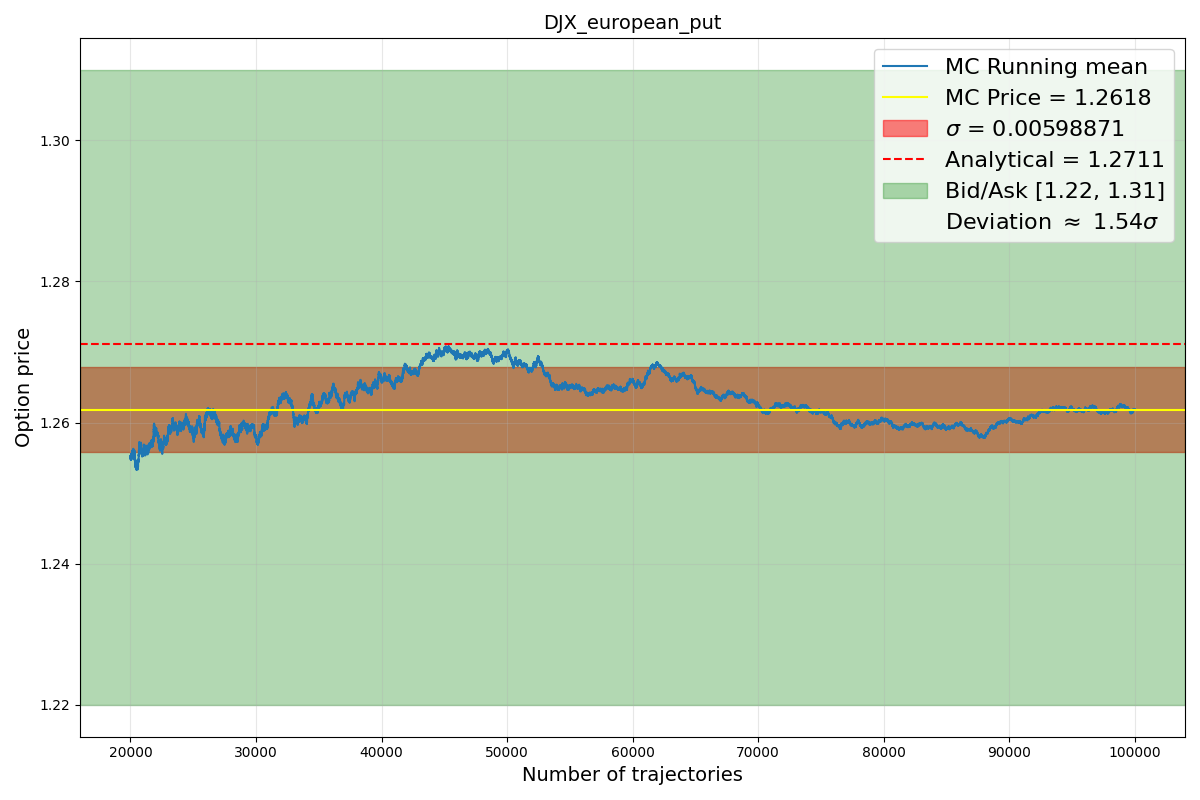
\includegraphics[width=\figw]{plots/DJX_european_put.png}
    \caption{DJX European put option with maturity date 2013-01-19, quoted on 2013-01-02; $S_0=134.13$, $X=134.0$, $r=0.01$, $\sigma=0.1183$, $T=17/365$; data from~\cite{optiondata}.}
    \label{eu-put}
\end{figure}
In Fig. \ref{eu-put} we see that for the given european put option we get a sensible price from the monte carlo simulation within $1.54\sigma$ of the estimated analytical solution, and well within the quoted bid/ask price of that day.
\begin{figure}[htbp]
    \centering
    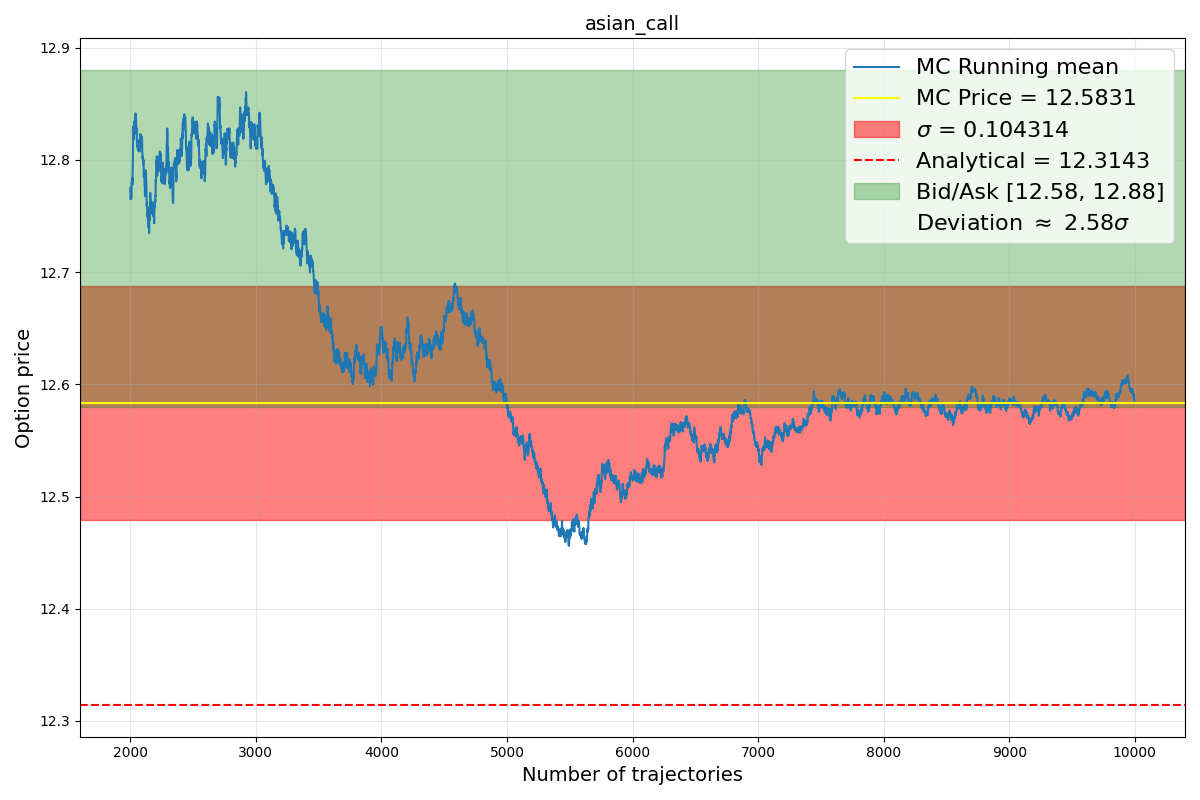
\includegraphics[width=\figw]{plots/asian_call.png}
    \caption{Asian call option; fictive bid/ask values are the max/min from the Monte Carlo reference in~\cite{divaAsian}; $S_0=100.0$, $X=0.90$, $r=0.05$, $\sigma=0.20$, $T=1$.}
    \label{asian-call}
\end{figure}
\begin{figure}[htbp]
    \centering
    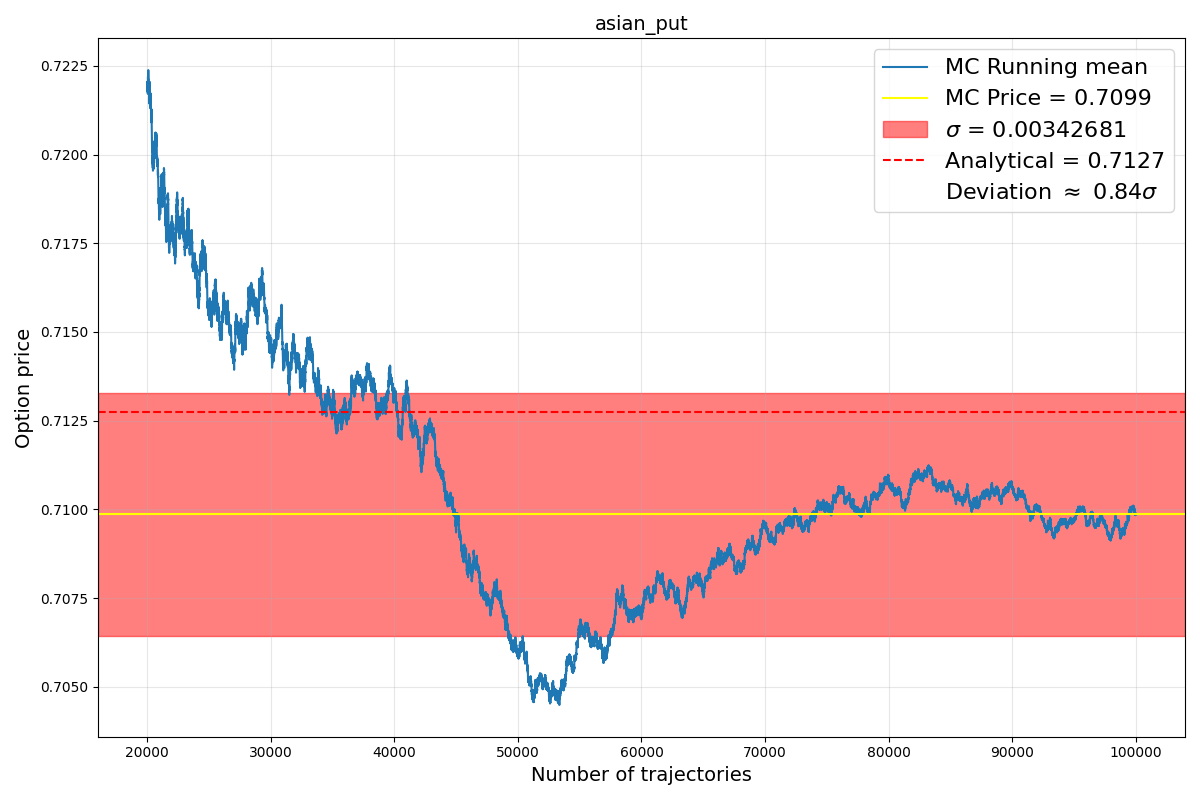
\includegraphics[width=\figw]{plots/asian_put.png}
    \caption{Asian put option, with parameters being the same ones as for the European Put but calculated as an asian option (i could not find free data), $S_0 = 134.13$, $X=134.0$, $r=0.01$, $\sigma = 0.1183$, $T=\frac{17}{365}$ }
    \label{asian-put}
\end{figure}
\begin{figure}[htbp]
    \centering
    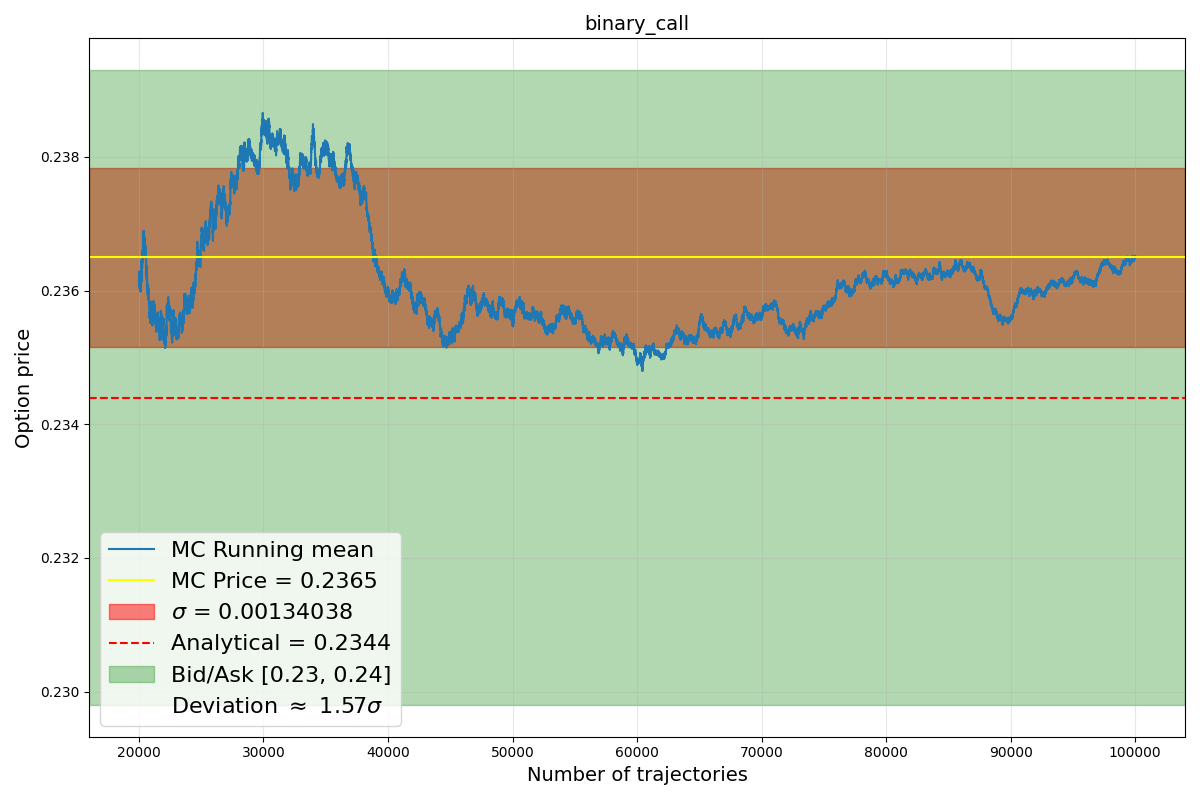
\includegraphics[width=\figw]{plots/binary_call.png}
    \caption{Binary call option; parameters taken from~\cite{eudlBinary}, whose result is $0.23458\pm 2\%$ (indicated as the fictive bid-ask range). $S_0=121.675$, $X=150$, $r=0.0156$, $\sigma=0.7860$, $T=90/365$; risk-free-rate is the 5-year treasury bill yield.}
    \label{binary-call}
\end{figure}
\begin{figure}[htbp]
    \centering
    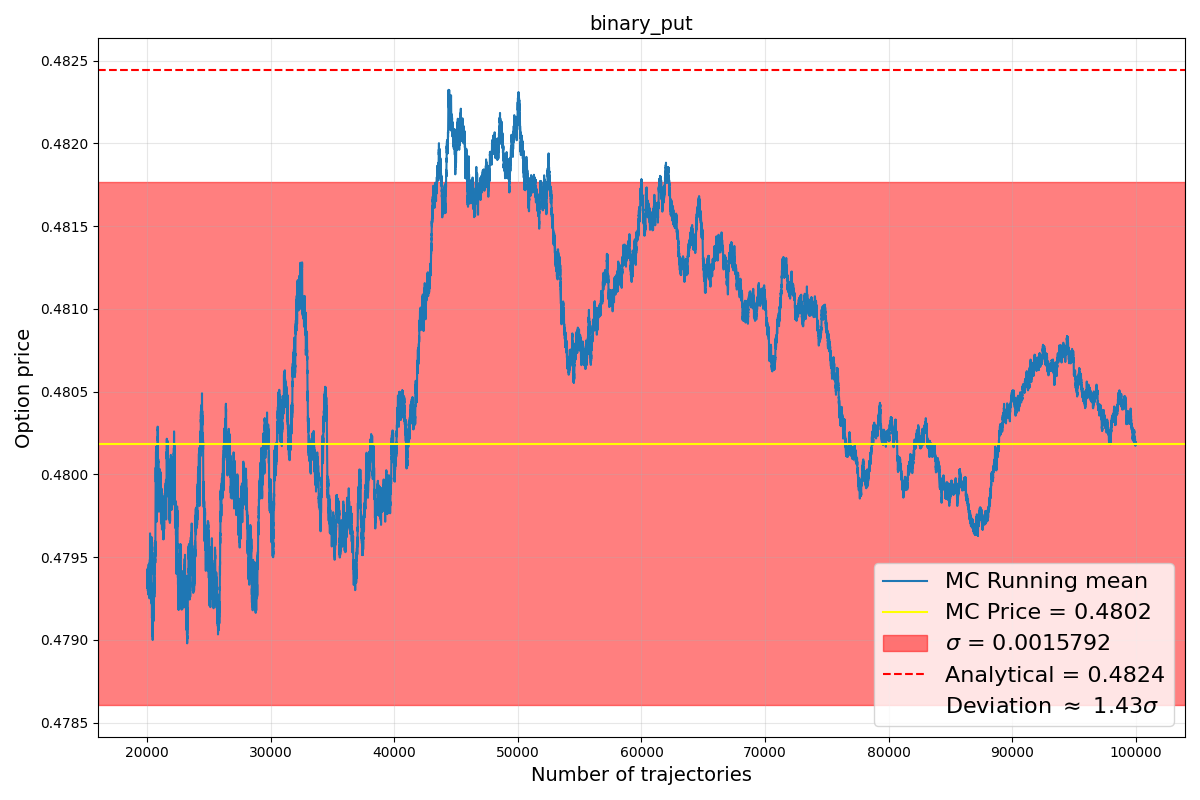
\includegraphics[width=\figw]{plots/binary_put.png}
    \caption{Binary put option, with parameters being the same ones as for the European Put but calculated as a binary put option (i could not find free data), $S_0 = 134.13$, $X=134.0$, $r=0.01$, $\sigma = 0.1183$, $T=\frac{17}{365}$ }
    \label{binary-put}
\end{figure}
\begin{figure}[htbp]
    \centering
    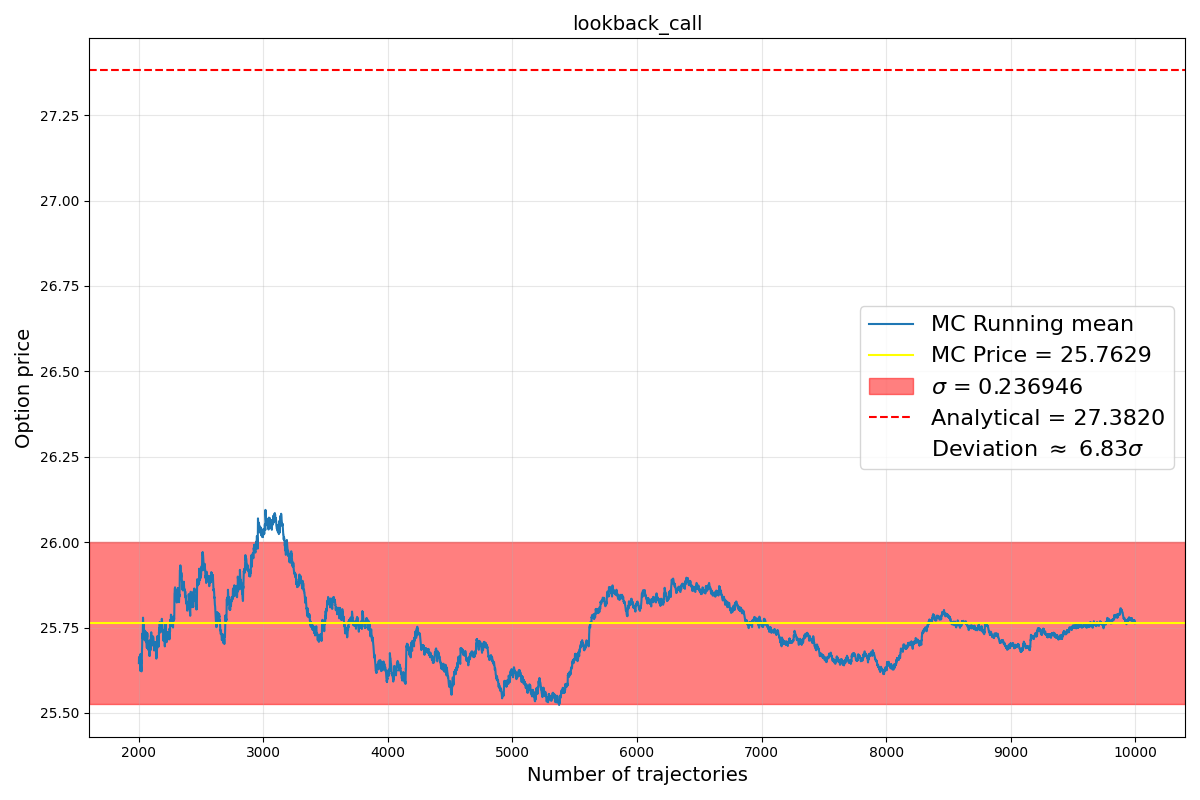
\includegraphics[width=\figw]{plots/lookback_call.png}
    \caption{Lookback call option with parameters from~\cite{quantstartLB}; the analytical formula assumes a minimum price $10\%$ below $S_0$. $S_0=100$, $r=0.1$, $\sigma=0.3$, $T=1$, $N_{MC}=10000$, $n_{steps}=10000$.}
    \label{lookback_call}
\end{figure}
\begin{figure}[htbp]
    \centering
    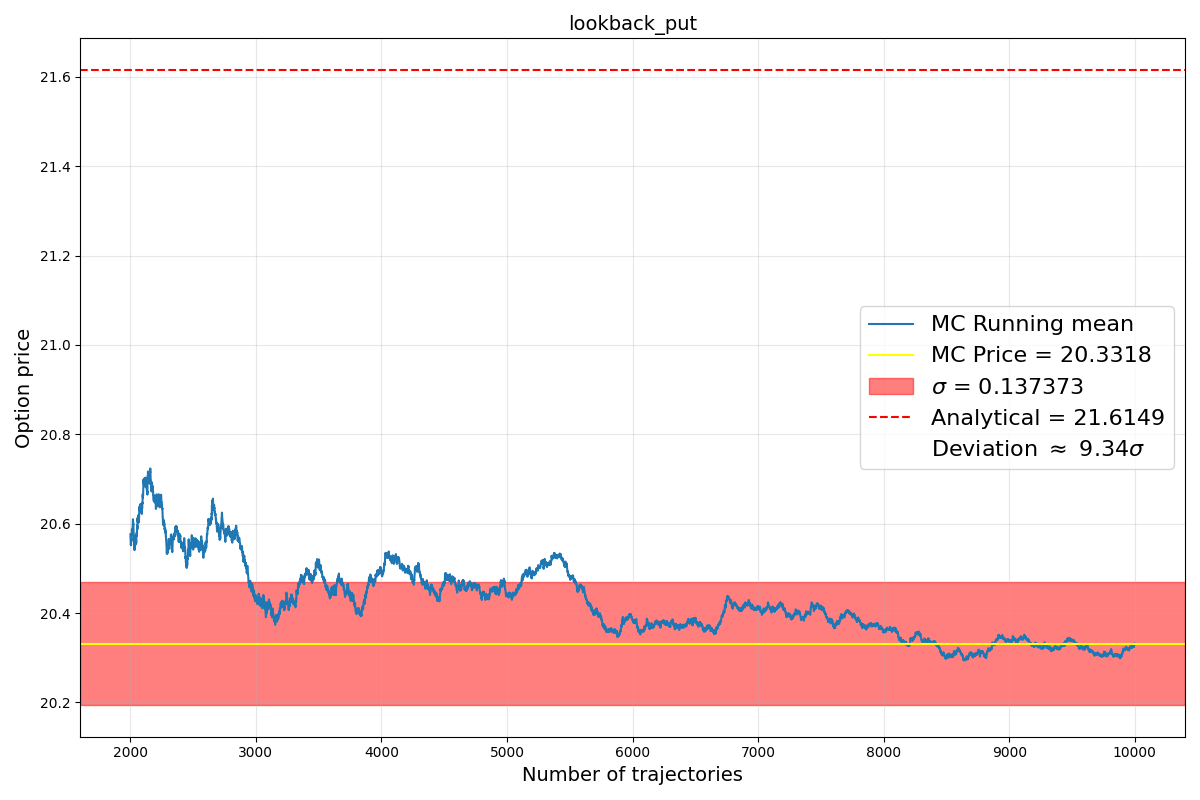
\includegraphics[width=\figw]{plots/lookback_put.png}
    \caption{Lookback put option with the same parameters as the above call option, the analytical equation assumes a max price of $10\%$ higher than $S_0$, $N_{MC}=10000$, $n_{steps}=10000$}
    \label{lookback_put}
\end{figure}
We realise that the Monte Carlo simulations seem to provide reasonable results; the results from both lookback options are poor, as one can see by the high deviation (in $\sigma$). However,~\cite{rgLB} reports that floating-strike lookback options do perform poorly in Monte Carlo simulations, with similar deviations from the analytical value.
One interesting fact is that the LookBack simulations seemed to perform better if the step size was increased, the bigger the better it seems.
\clearpage
\section{Black--Scholes as a Diffusion Equation: Derivation}

We have the Black-Scholes equation:
\begin{equation}
    \frac{\partial C}{\partial t} + \frac{1}{2} \sigma^2 S^2 \frac{\partial^2 C}{\partial S^2} + rS \frac{\partial C}{\partial S} - rC = 0
    \label{eq:bs}
\end{equation}
with the following boundary conditions:
\begin{equation}
    C(S,T)=\max(S-X,0) \tag{1}
    \label{eq:cond1}
\end{equation}
\begin{align}
    & C(0,t)=0,
    & \lim_{S\to\infty}C(S,t)\propto S.
    \label{eq:boundaryconditions}
\end{align}
We rewrite Eq. \ref{eq:bs} in the following way:
\begin{equation}
    \frac{\partial C}{\partial t} + \frac{1}{2} \sigma ^2 (S \frac{\partial}{\partial S})^2 C + (r - \frac{1}{2}\sigma^2) S \frac{\partial C}{\partial S} - rC = 0
    \label{eq:bs2}
\end{equation}
We introduce the following change of variables:
\begin{align}
    & S = e^y
    & t = T - \tau
\end{align}
This change of variables is motivated by the fact, that the underlying process described by S is a geometric Brownian motion (that's how the stock price behaves). That way $y=\log{S}$ describes a Brownian motion (with a possible drift).\\
Secondly the evolution of the system is backwards from the terminal state of the system, thus we have to reverse time.\\
This results in
\begin{align}
    &S \frac{\partial}{\partial S} \rightarrow \frac{\partial}{\partial y},
    & \frac{\partial}{\partial t} \rightarrow - \frac{\partial}{\partial \tau}
\end{align}
giving us a new form of Eq. \ref{eq:bs2}:
\begin{equation}
    \frac{\partial C}{\partial \tau} - \frac{1}{2} \sigma ^2 \frac{\partial^2 C}{\partial y^2} - (r - \frac{1}{2}\sigma^2) \frac{\partial C}{\partial y} + rC = 0
    \label{eq:bs3}
\end{equation}
Now we see that if we were to get rid of the last two terms, we would have a diffusion equation.\\
Next we discount the option price $C$ with (remember $\tau \propto -t$)
\begin{equation}
    u(y,\tau) = e^{r\tau} C(y,\tau)
    \label{eq:subu}
\end{equation}
This substitution then leads (due to the chain rule) $\frac{\partial e^{-r\tau} u}{\partial \tau} = -r e^{-r\tau}u + e^{-r\tau} \frac{\partial u}{\partial \tau}$ and helps us to get rid of the previous $rC$ term. We receive the following equation:
\begin{equation}
    \frac{\partial u}{\partial \tau} - \frac{1}{2}\sigma^2 \frac{\partial^2 u}{\partial y^2} - (r - \frac{1}{2} \sigma^2) \frac{\partial u}{\partial y} = 0
    \label{eq:bs4}
\end{equation}
Now we are left with a single partial derivative with respect to $y$. This one does not cancel yet, unless $r=\frac{1}{2}\sigma^2$ because we have not taken into account the drift of the Brownian motion. The drift is linear in time $\tau$, thus we can make the following substitution:
\begin{align}
    & x = y + (r - \frac{1}{2}\sigma^2) \tau,
    & \tau = t
\end{align}
We then receive an equation of form:
\begin{equation}
    \frac{\partial u}{\partial \tau} = \frac{1}{2}\sigma^2 \frac{\partial^2 u}{\partial x^2}
    \label{eq:diffusion}
\end{equation}
The function $u(x,\tau)$ is defined for $-\infty < x < \infty$ and $0 \leq \tau \leq T$. The terminal condition Eq. \ref{eq:cond1} of the original Black-Scholes problem becomes the initial condition of the heat equation at $\tau=0$. The substitutions we did so far ($u=e^{r\tau}C$ and $x = y + (r-\frac{1}{2}\sigma^2)\tau$) reduce at $\tau=0$ to the identity ($u=C$, $x = y = \log S$), so the initial condition is simply the call payoff written in the new variable $x$:
\begin{equation}
    u(x,0) = u_0(x) = \max(e^x - X,\,0).
    \label{eq:ic}
\end{equation}
This is just the standard $\max(S-X,0)$ payoff, evaluated at $S = e^x$.\\
The solution of the equation is given by the known solution of the heat equation:
\begin{equation}
    u(x,\tau) = \frac{1}{\sigma \sqrt{2\pi \tau}} \int_{-\infty}^{\infty} u_0 (s) e^{-\frac{(x-s)^2}{2\sigma^2 \tau}} ds
\end{equation}
We can evaluate this integral and then return to the former variables $(x, \tau, u)$ $\rightarrow$ $(S,t,C)$ via
\begin{equation}
    C(S,t) = e^{-r\tau}\, u\bigl(\log S + (r - \tfrac{1}{2}\sigma^2)\tau,\;\tau\bigr),\qquad \tau = T-t.
    \label{eq:inversion}
\end{equation}

\section{Numerical Approach for the Diffusion Equation}
Now we want to solve the diffusion equation numerically, for the Black Scholes model. \\
We choose a spatial domain $x \in \left[x_{min}, x_{max} \right]$ and discretize it into $L$ grid points with spacing $\Delta x$.\\
Let
\begin{equation}
    u_i(\tau) = u(x_i, \tau), \qquad i=1,\cdots,L
    \label{eq:uapprox}
\end{equation}
so that essentially it becomes a vector like
\begin{equation} \vec{u}(\tau) =
    \begin{pmatrix}
        u_1(\tau)\\
        \vdots\\
        u_L(\tau)
    \end{pmatrix}
    \label{eq:uvector}
\end{equation}
The time evolution now happens by updating this vector within the numerical simulation.\\
Looking at Eq. \ref{eq:diffusion}, we realize that we have a second derivative, we use the standard central difference to rewrite it as:
\begin{equation}
    \frac{\partial ^2 u(x, \tau)}{\partial x^2} \approx \frac{\frac{u_{i+1} - u_i}{\Delta x} - \frac{u_{i} - u_{i-1}}{\Delta x}}{\Delta x} \approx \frac{u_{i+1} - 2u_i + u_{i-1}}{(\Delta x)^2}
    \label{eq:numeric1}
\end{equation}
We can go further by writing out the full diffusion equation:
\begin{equation}
    \frac{\partial u(x,\tau)}{\partial \tau} = D  \frac{u_{i+1} - 2u_i + u_{i-1}}{(\Delta x)^2}
\end{equation}
where we defined $D=\frac{\sigma^2}{2}$.\\
Now for the full grid we can rewrite this equation using a matrix, calling it $\hat{H}$
\begin{equation}
\hat{H}=
\begin{bmatrix}
    2 & -1 & 0 & . & . & . &  0 &  \\
    -1 & 2 & -1 &   &   &   &  . &   \\
    0 & -1 & 2 &   &   &   &  . &   \\
    . &   &    & . &   &   &  . &   \\
    . &   &    &   & . &   &  0 &   \\
    . &   &    &   &   & 2 &  -1 &   \\
    0 & . &  . & . & 0 & -1 & 2 &   \\
\end{bmatrix}
\label{D-matrix}
\end{equation}
to be of form:
\begin{equation}
    \frac{\partial \vec{u}(\tau)}{\partial \tau} = -\frac{D}{(\Delta x)^2}\hat{H} \vec{u}(\tau)
    \label{eq:diffusion_new}
\end{equation}
The matrix $\hat{H}$ can then be decomposed into the two matrices \\
\begin{minipage}{0.6\textwidth}
\begin{equation*}
\hat{A}=
\begin{bmatrix}
    1 & -1 & 0 & . & . & . &  0 &  \\
    -1 & 1 & 0 &   &   &   &  . &   \\
    0 & 0 & 1 & -1 &   &   &  . &   \\
    . &   & -1 & . &   &   &  . &   \\
    . &   &    &   & . &   &  0 &   \\
    . &   &    &   &   & 1 &  -1 &   \\
    0 & . &  . & . & 0 & -1 & 1 &   \\
\end{bmatrix}
\;\text{and}\;
\label{A-matrix}
\end{equation*}
\end{minipage}
\begin{minipage}{0.5\textwidth}
\begin{equation*}
\hat{B}=
\begin{bmatrix}
    1 & 0 & 0 & . & . & . &  0 &  \\
    0 & 1 & -1 &   &   &   &  . &   \\
    0 & -1 & 1 &   &   &   &  . &   \\
    . &   &    & . &   &   &  . &   \\
    . &   &    &   & . & -1  &  0 &   \\
    . &   &    &   &  -1 & 1 &  0 &   \\
    0 & . &  . & . & 0 & 0 & 1 &   \\
\end{bmatrix}
\label{B-matrix}
\;\text{.}
\end{equation*}
\end{minipage}\\ \\
So it means now that $\hat{H} = \hat{A} + \hat{B}$ and that the solution to our diffusion Eq. \ref{eq:diffusion_new} is then (with $\alpha = -\frac{D}{(\Delta x)^2}$):
\begin{equation}
    \vec{u}(\tau + \Delta_\tau) = e^{\alpha \hat{H} \Delta_\tau} \vec{u}(\tau)
    \label{eq:solve1}
\end{equation}
where $\Delta_\tau$ is the size of one numerical time step.\\
Now since $\hat{H}$ is neither diagonal nor block-diagonal, we do not really know how the exponential looks, and also since these are matrices and not numbers, generally $e^{\hat{H}} \neq e^{\hat{A}}e^{\hat{B}}$, but using the Lie--Trotter product formula, to first order (see~\cite{strangSplitting}):
\begin{equation}
    e^{t(\hat{A}+\hat{B})} = \lim_{n\to\infty} (e^{t\hat{A}/n} e^{t\hat{B}/n})^n
\end{equation}
we can approximate to second order the exponential of the matrices (the proof is done via some steps involving the Baker-Campbell-Hausdorff formula since the matrices don't commute) such that we get the second order product formula (Strang splitting):
\begin{equation}
    e^{\alpha \hat{H}\,\Delta_\tau} \;\approx\; e^{\tfrac{1}{2}\alpha \hat{A}\,\Delta_\tau}\; e^{\alpha \hat{B}\,\Delta_\tau}\; e^{\tfrac{1}{2}\alpha \hat{A}\,\Delta_\tau}.
    \label{eq:strang}
\end{equation}
Finally the full time evolution for our system over the total interval $T$ is then done by applying this time-stepping formula $m$ times, with $\Delta_\tau = T/m$:
\begin{equation}
    e^{\alpha \hat{H}\,T} \;\approx\; \left( e^{\tfrac{1}{2}\alpha \hat{A}\,\Delta_\tau}\; e^{\alpha \hat{B}\,\Delta_\tau}\; e^{\tfrac{1}{2}\alpha \hat{A}\,\Delta_\tau} \right)^{m}.
    \label{eq:solve2}
\end{equation}
The diffusion equation can then be solved by \ref{eq:solve1}, with the usage of \ref{eq:solve2}.
The matrix exponential of a block diagonal matrix, where each block is of the form
$
\hat{X}=
\begin{bmatrix}
     1 & -1 \\
    -1 & 1  \\
\end{bmatrix}
$, can be easily determined by computing
\begin{equation}
    e^{q\hat X}=\sum_{k=0}^{\infty} \frac{q^k}{k!}\hat X^k = \mathbf{1}+\frac{\hat{X}}{2}(e^{2q}-1)
\end{equation}
where $\mathbf{1}$ defines the identity matrix.\\
Practically in my simulation $\hat{A}$ and $\hat{B}$ are block-diagonal $L\times L$ matrices where the first block of $\hat{B}$ and the last block of $\hat{A}$ are $1\times 1$ unity blocks, and the rest are $2\times 2$ blocks of the form $\hat{X}$ above. Reading off the half-step exponent from Eq. \ref{eq:strang}, the half-step factor for $\hat{A}$ is $e^{\tfrac{1}{2}\alpha\Delta_\tau\hat{X}}$ and the full-step factor for $\hat{B}$ is $e^{\alpha\Delta_\tau\hat{X}}$. Defining the dimensionless number
\begin{equation}
    \beta \;=\; \alpha\,\Delta_\tau \;=\; -\frac{D\,\Delta_\tau}{\Delta x^{2}},
    \label{eq:beta}
\end{equation}
the per-block matrices that appear in the Strang substep are
\begin{align}
    e^{(\beta/2)\hat{X}} &= \frac{1}{2}\begin{bmatrix}
         1 + e^{\beta} & 1-e^{\beta} \\
        1-e^{\beta} & 1 + e^{\beta}
    \end{bmatrix}\quad \text{(half-step for $\hat A$)},\\
    e^{\beta\hat{X}}   &= \frac{1}{2}\begin{bmatrix}
         1 + e^{2\beta} & 1-e^{2\beta} \\
        1-e^{2\beta} & 1 + e^{2\beta}
    \end{bmatrix}\quad \text{(full-step for $\hat B$)},
\end{align}
and the lone $1\times 1$ blocks at the corners pick up $e^{\beta/2}$ (for the last block of $\hat A$) and $e^{\beta}$ (for the first block of $\hat B$), respectively. In the code these matrices are constructed once, and the Strang substep is applied $m$ times in the time loop.\\
Finally in order to be able to write our simulation, we need to define the correct intial conditions with the transformed variables. From Eq. \ref{eq:ic} we already have the initial condition in closed form,
\begin{equation}
    u_i (0) = \max\!\bigl(e^{x_i} - X,\,0\bigr),
    \label{eq:boundary1}
\end{equation}
which is just the call payoff evaluated at the grid points $S_i = e^{x_i}$. This means that each grid point will have the value $u_i(0)$ assigned to it at the beginning of the simulation. The variable $x$ is directly related to $S$ as it is defined as $x = \log{S} + (r - \frac{1}{2}\sigma^2)\tau$, which directly denies the possibility of having a stock price $S=0$. So i chose $S_{min}$ and $S_{max}$ to lie well away from the strike $X$, with $S_{min}$ a small fraction of $X$ and $S_{max}$ several multiples of $X$. With these values for $S$ i calculate the max and min value for $x$ and space them equally on a grid of $L=1001$ points, where $\Delta x$ is the difference between each point.\\
During the simulation we also have to make sure that the boundary conditions are correct. For the left boundary ($S\rightarrow 0$) we have
\begin{align}
    C(0,t) = 0 \quad \rightarrow \quad \lim_{x\to -\infty}u(x,\tau) = 0,
\end{align}
so $u_1(\tau)=0$ throughout the simulation.\\
For the right boundary ($S\rightarrow\infty$), we know that for large $S$ the call price behaves as $C(S,t)\sim S - X e^{-r(T-t)}$. Plugging this into $u = e^{r\tau}C$ together with $S = e^{x-(r-\sigma^2/2)\tau}$ gives
\begin{equation}
    u(x_{\max},\tau) \;\sim\; e^{\,x_{\max} + \tfrac{1}{2}\sigma^{2}\tau} - X.
    \label{eq:rightBC}
\end{equation}
At every time step we set $u_L(\tau)$ to this asymptote.

\subsection{Results}
With the initial condition Eq.~\eqref{eq:boundary1}, the Strang split Eq.~\eqref{eq:solve2}, the $\beta$ from Eq.~\eqref{eq:beta} and the boundary conditions above, the numerical solver reproduces the analytical Black--Scholes price to within the spatial discretisation error of $\mathcal{O}(\Delta x^{2})$.

We test it on the BKX European call from the Monte Carlo section, using the exact same parameters ($S_0=52.93$, $X=37.5$, $r=0.01$, $\sigma=0.1586$, $T=17/365$). Fig.~\ref{diffusion} shows the numerical curve $C(S,0)$ from the diffusion solver overlaid on the analytical Black--Scholes price. The two curves are visually indistinguishable; at $S=S_0$ the numerical price is $15.388$ versus an analytical $15.448$, a relative deviation of $0.4\%$. This is well within the quoted bid--ask spread ($13.1/17.4$) for that day.

\begin{figure}[htbp]
    \centering
    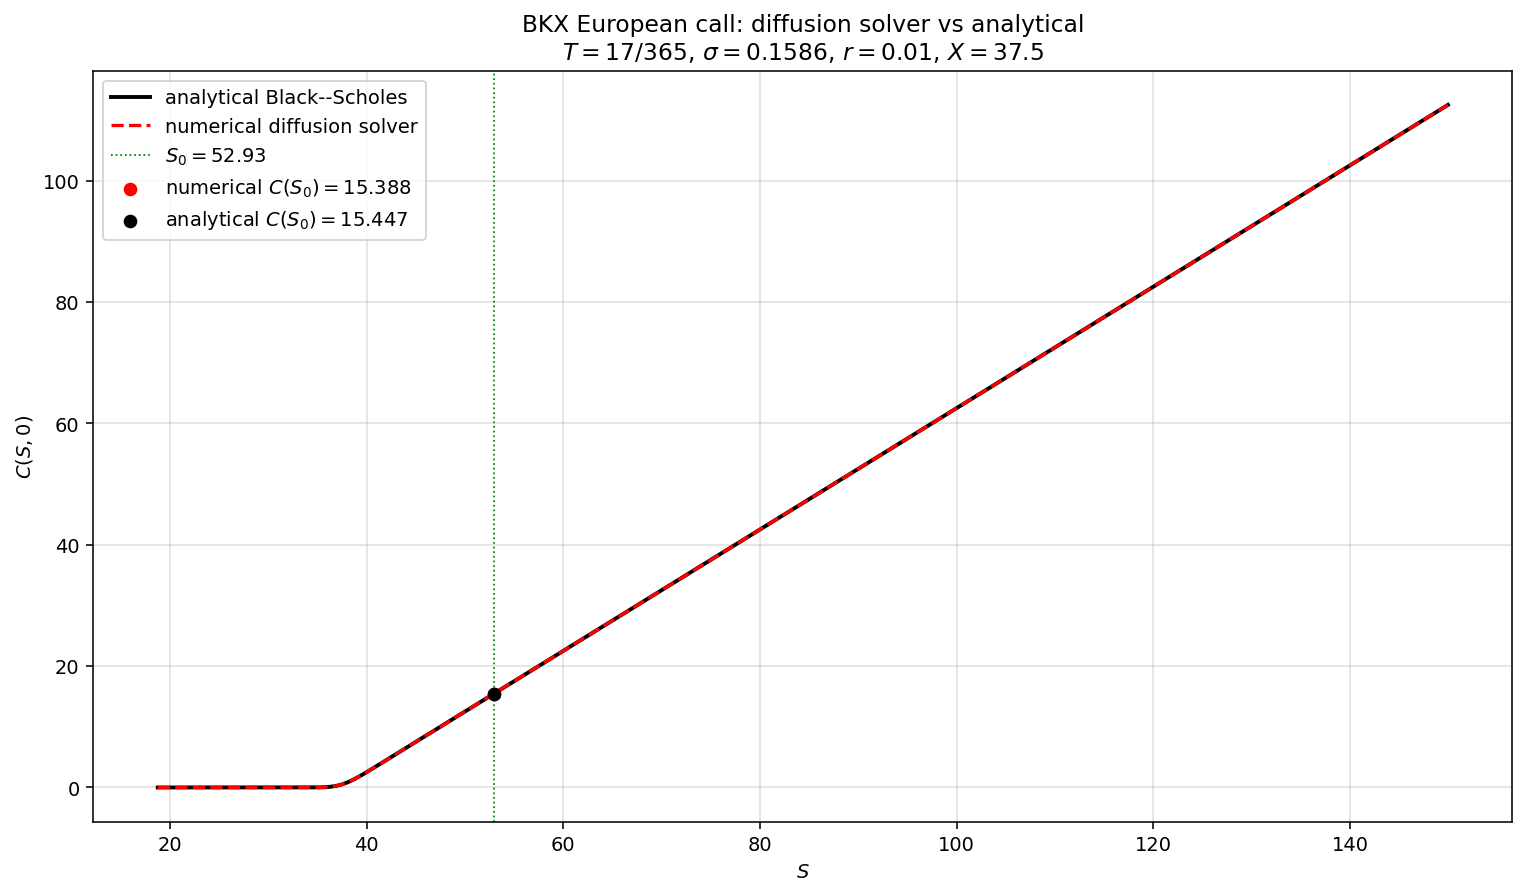
\includegraphics[width=\figwide]{plots/diffusion_BKX.png}
    \caption{BKX European Call: numerical price $C(S,0)$ from the diffusion solver (red dashed) overlaid on the analytical Black--Scholes price (black). Markers indicate the value at $S_0$. Bid: 13.1, Ask: 17.4; $S_0=52.93$, $X=37.5$, $r=0.01$, $\sigma=0.1586$, $T=17/365$; data from~\cite{optiondata}.}
    \label{diffusion}
\end{figure}

Because the BKX maturity is only $T=17/365\approx 0.047$, the heat-equation evolution barely has time to smooth the kink of the payoff, and the surface $C(S,t)$ is almost the payoff itself. To actually see the diffusion at work, i also ran the same solver on a textbook-style set of parameters $T=1$, $\sigma=0.30$, $r=0.05$, $X=100$, where the kink has plenty of time to smooth out. Fig.~\ref{diff-compare} shows the resulting numerical surface side-by-side with the analytical Black-Scholes surface, and Fig.~\ref{diff-overlay} overlays the numerical samples (red dots) on the analytical surface (smooth colormap) to emphasise that the two agree pointwise.

\begin{figure}[htbp]
    \centering
    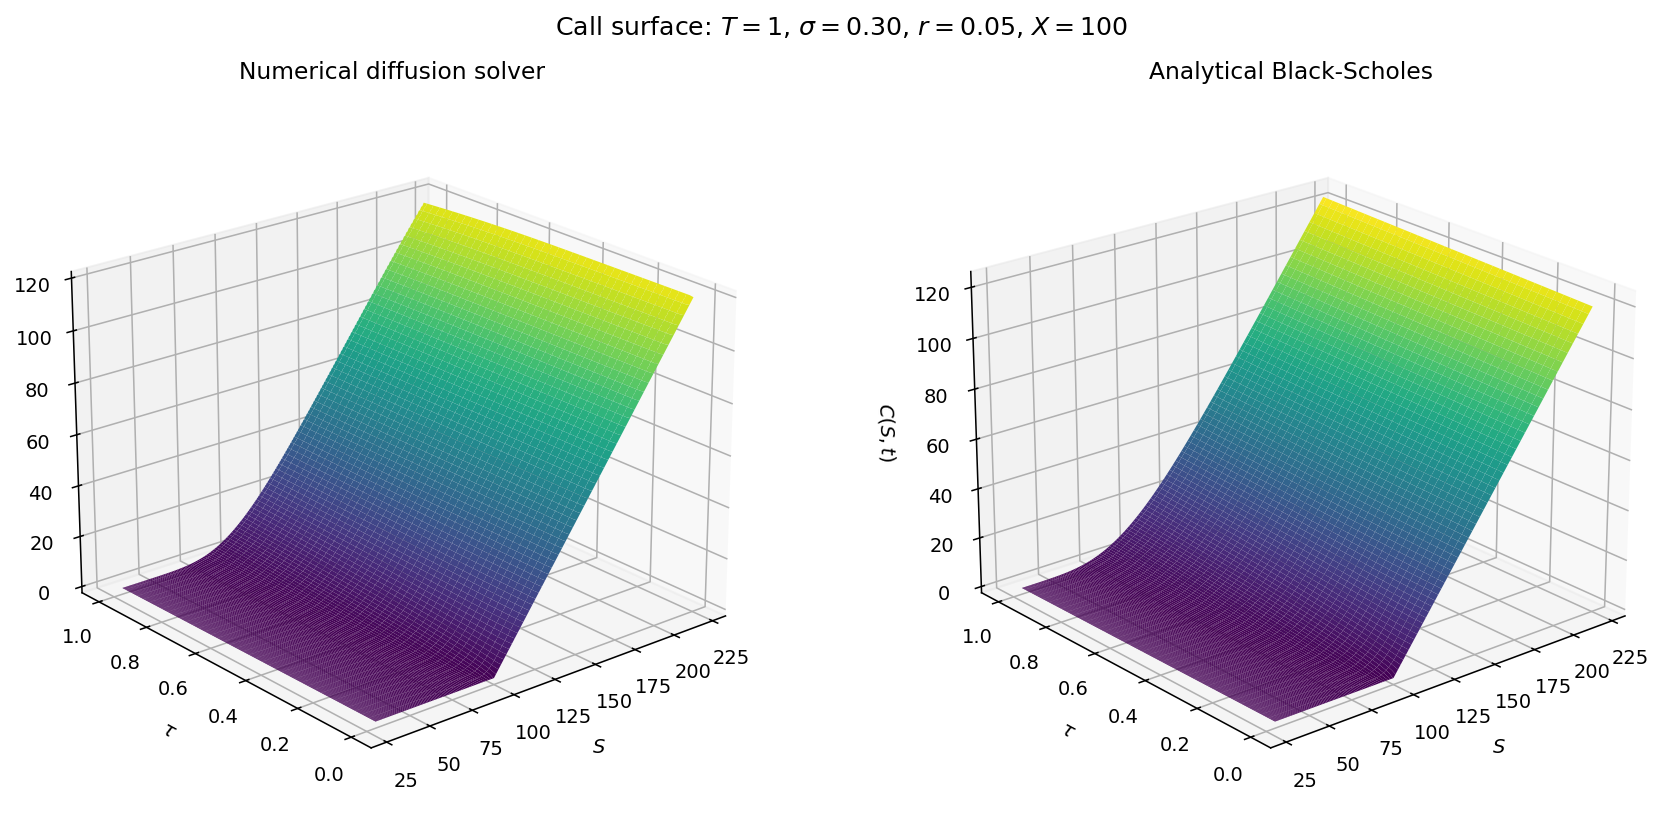
\includegraphics[width=\figwide]{plots/diffusion_compare.png}
    \caption{Call-price surface $C(S,t)$ versus $S$ and $\tau=T-t$ from the diffusion solver (left) compared with the analytical Black-Scholes surface (right). Parameters: $T=1$, $\sigma=0.30$, $r=0.05$, $X=100$.}
    \label{diff-compare}
\end{figure}

\begin{figure}[htbp]
    \centering
    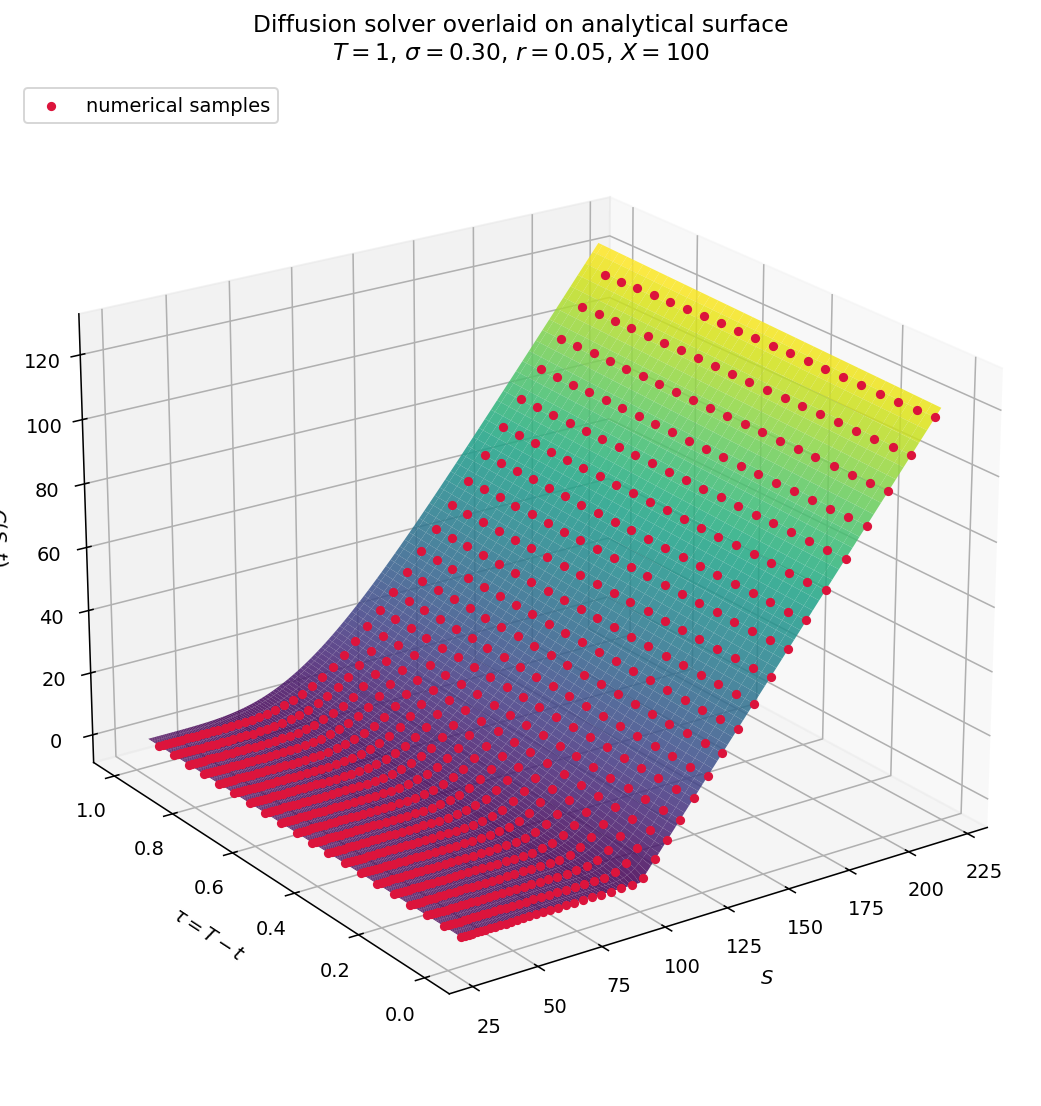
\includegraphics[width=\figw]{plots/diffusion_overlay.png}
    \caption{Same data as Fig.~\ref{diff-compare}: numerical samples (red dots) overlaid on the analytical surface. The samples sit on the surface, which is what we want.}
    \label{diff-overlay}
\end{figure}

To get a quantitative feel for the agreement, Fig.~\ref{diff-slices} shows three slices at $\tau=0$ (the payoff), $\tau=0.25$ and $\tau=1$ (deep into maturity). At $\tau=0$ the numerical curve sits exactly on the kinked payoff, as it should -- this is the initial condition Eq.~\ref{eq:boundary1} verbatim. At intermediate $\tau$ the curves agree to the eye. At $\tau=1$ there is a small undershoot at large $S$; this comes from imposing the finite-$x_{\max}$ asymptote Eq.~\ref{eq:rightBC} on a truncated grid, and shrinks if one pushes $x_{\max}$ further out. Fig.~\ref{diff-error} shows the pointwise error $C_{\text{num}} - C_{\text{BS}}$ on the same grid; the error is everywhere small compared to the price level and is concentrated near the right boundary at late $\tau$, exactly where one expects it.

\begin{figure}[htbp]
    \centering
    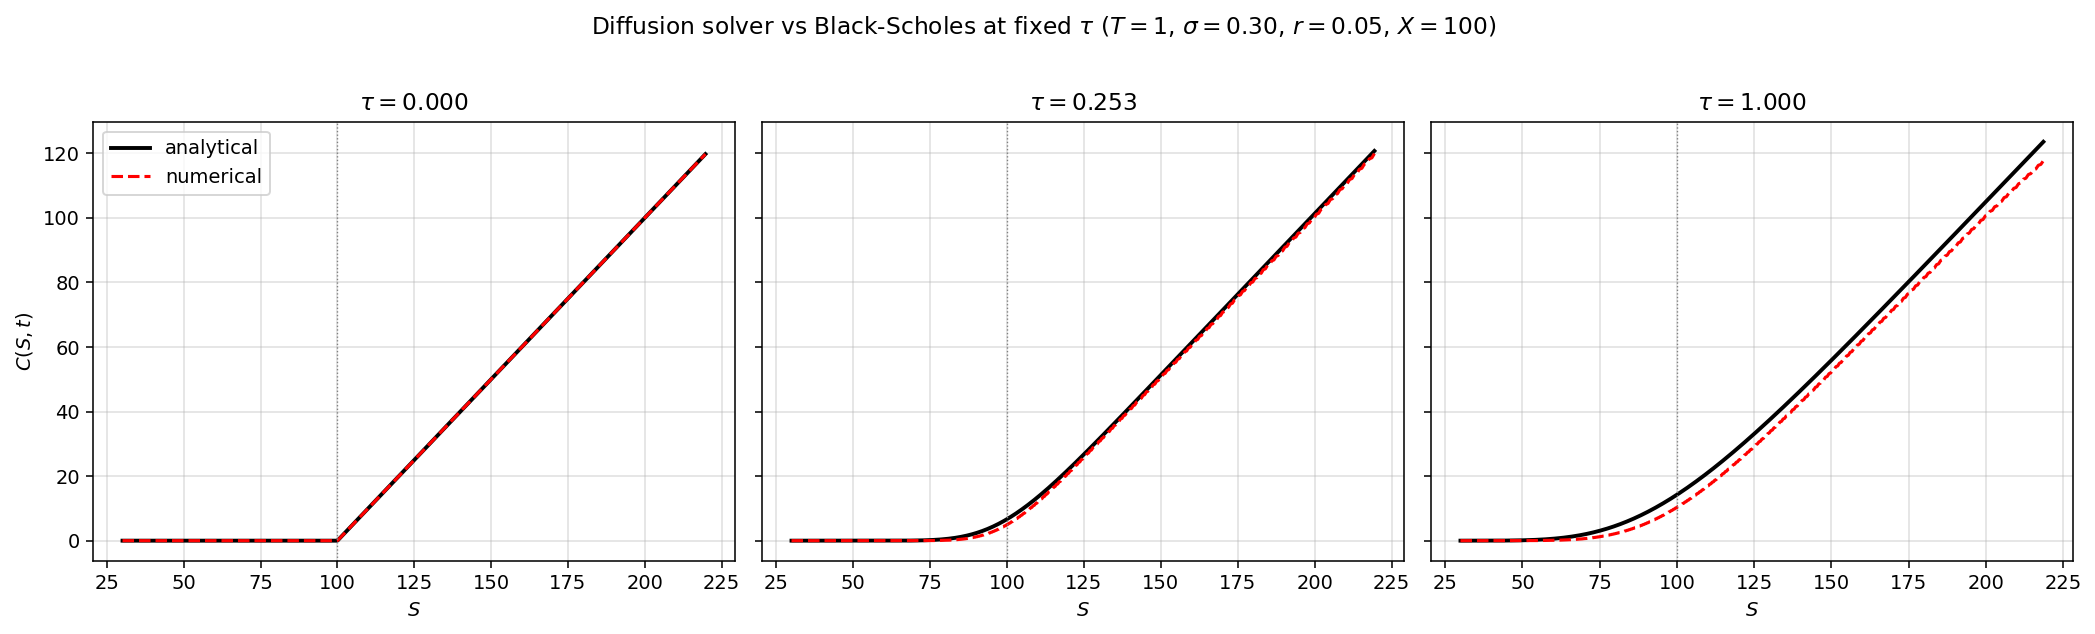
\includegraphics[width=\figwide]{plots/diffusion_slices.png}
    \caption{Slices of $C(S,t)$ at three values of $\tau$ for the $T=1$ benchmark. Black: analytical Black-Scholes; red dashed: diffusion solver. The dotted vertical line marks $S=X$.}
    \label{diff-slices}
\end{figure}

\begin{figure}[htbp]
    \centering
    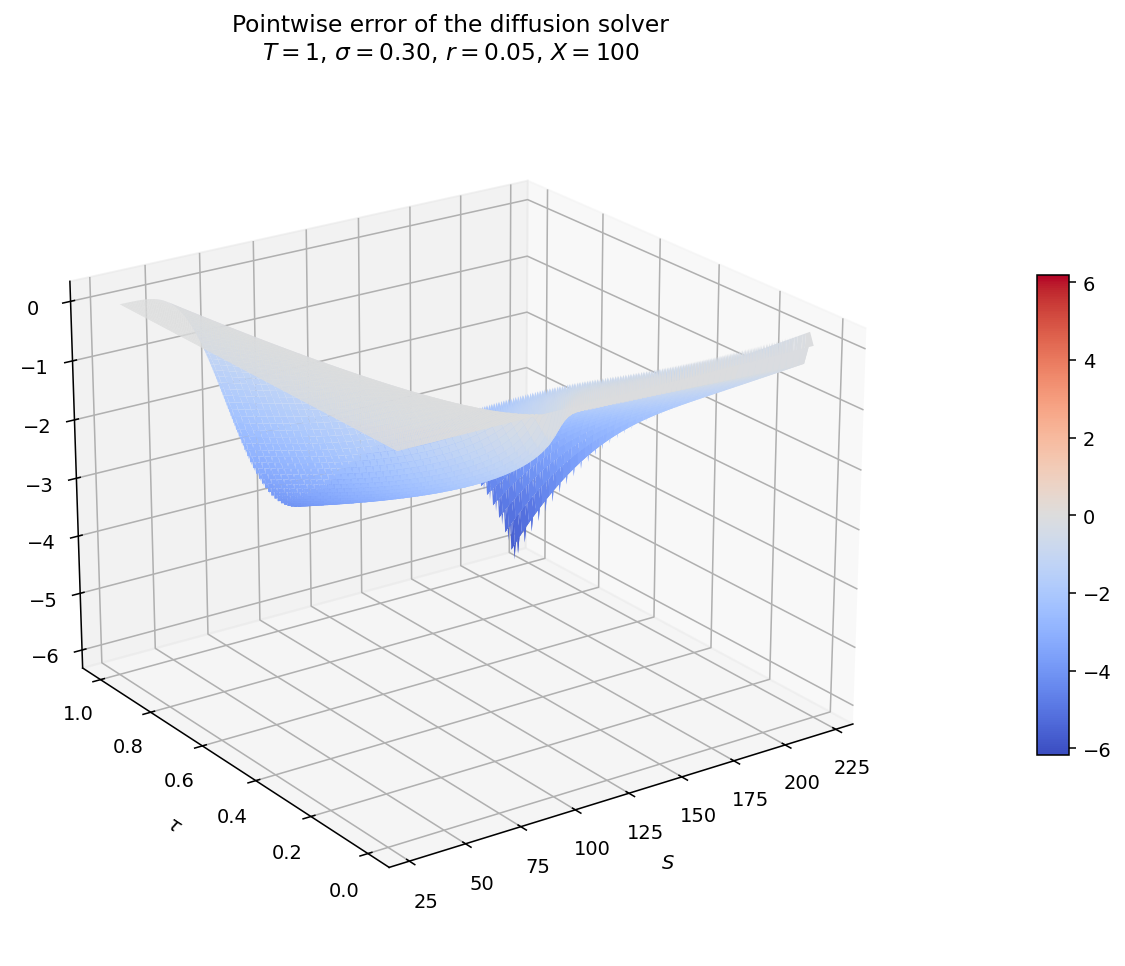
\includegraphics[width=\figwide]{plots/diffusion_error.png}
    \caption{Pointwise error $C_{\mathrm{num}}-C_{\mathrm{BS}}$ on the same $(S,\tau)$ grid as Fig.~\ref{diff-compare}. The error is small in magnitude and concentrated near the truncated right boundary at large $\tau$.}
    \label{diff-error}
\end{figure}

Overall the diffusion-equation solver agrees with the analytical Black-Scholes price across the whole $(S,\tau)$ surface within the expected $\mathcal{O}(\Delta x^{2})$ discretisation error, both for the short-maturity BKX option used in the Monte Carlo section and for the longer-maturity benchmark $T=1$.

\clearpage
\section*{AI Usage}
\addcontentsline{toc}{section}{AI Usage}
Claude Opus (Anthropic) was used to (i) refine the writing style of this report, (ii) resolve a numerical issue in the diffusion-equation solver where the discretised time step in the Strang splitting was mis-scaled, and (iii) generate the three-dimensional comparison plots (Figs.~\ref{diff-compare}, \ref{diff-overlay} and \ref{diff-error}) as well as the slice plot in Fig.~\ref{diff-slices}. The physics content, the derivations, the Monte Carlo implementation and the analytical formulae are my own; the AI tool acted as an editing and plotting assistant.

\clearpage
\begin{thebibliography}{9}
    \bibitem{optiondata}
    Historical option data,
    \url{https://optiondata.org}.

    \bibitem{divaAsian}
    T.~Aspenberg and V.~Nord,
    \emph{The Discrete Arithmetic Asian Option and a Comparison of Novel Methods for its Valuation},
    Bachelor Thesis, Uppsala Universitet, 2010.
    \url{https://www.diva-portal.org/smash/get/diva2:301070/FULLTEXT01.pdf}.

    \bibitem{quantstartLB}
    QuantStart,
    \emph{Floating-Strike Lookback Option Pricing with C++ via Analytic Formulae}.
    \url{https://www.quantstart.com/articles/Floating-Strike-Lookback-Option-Pricing-with-C-via-Analytic-Formulae}.

    \bibitem{eudlBinary}
    T.~L.~Nguyen and V.~T.~Pham,
    \emph{On Binary Option Pricing under the Black--Scholes Model},
    EAI Endorsed Transactions, 2022.
    \url{https://eudl.eu/pdf/10.4108/eai.28-10-2022.2328425}.

    \bibitem{rgLB}
    S.~Yadav,
    \emph{Estimating Lookback Price Using Monte Carlo Simulation and Binomial Lattice}, 2021.
    \url{https://www.researchgate.net/publication/351788645}.

    \bibitem{strangSplitting}
    Strang splitting (background reference).
    \url{https://grokipedia.com/page/Strang_splitting}.
\end{thebibliography}

\end{document}
